\section{LEVEL 1 · Centrummaten}

\begin{missie}
Missie: zoek het ‘centrum’ van je data.
\end{missie}

\begin{doel}
\textbf{DOEL} \quad Na dit level kan je:

☐ het \textbf{gemiddelde}, de \textbf{mediaan} en de \textbf{modus} berekenen en in een zin interpreteren;

☐ bepalen welke centrummaat bij welk soort data past;

☐ uitleggen wat een \textbf{uitschieter} doet met het gemiddelde en met de mediaan;

☐ het gemiddelde schatten uit een \textbf{gegroepeerde frequentietabel}.
\end{doel}

\subsection*{Theorie 1.1 · Gemiddelde, mediaan en modus}

\begin{theorie}
Een \textbf{centrummaat} is een kengetal dat het centrum van een gegevensreeks weergeeft.

\begin{itemize}
\item \textbf{Gemiddelde}: de som van alle gegevens gedeeld door het aantal gegevens. Steekproef: $\overline{x}=\dfrac{x_1+x_2+\dots+x_n}{n}$. Populatie: $\mu=\dfrac{x_1+x_2+\dots+x_N}{N}$. Rond af op één decimaal méér dan de data.
\item \textbf{Mediaan} (Med): de middelste waarde als je de data rangschikt van klein naar groot. Bij een \emph{even} aantal gegevens neem je het gemiddelde van de twee middelste. De helft van de gegevens is kleiner of gelijk aan de mediaan, de andere helft groter of gelijk.
\item \textbf{Modus} (Mod): de waarde die het vaakst voorkomt. Er kunnen meerdere modi zijn, of geen enkele als alle waarden even vaak voorkomen.
\end{itemize}

Welke centrummaat kan je gebruiken?

\breedtes{40/20/20/20}
\begin{tabular}{lccc}
\hline
soort data & gemiddelde & mediaan & modus \\
\hline
numeriek & ✔ & ✔ & ✔ \\
categorisch geordend & ✘ & ✔ & ✔ \\
categorisch niet-geordend & ✘ & ✘ & ✔ \\
\hline
\end{tabular}
\end{theorie}

\begin{voorbeeld}
\textbf{Voorbeeld.} Negen kinderen leenden dit jaar het volgende aantal boeken uit in de bib: 15, 9, 12, 15, 21, 10, 18, 15, 11.

\textbf{Stap 1: rangschikken.} 9 – 10 – 11 – 12 – \textbf{15} – 15 – 15 – 18 – 21

\textbf{Gemiddelde:} $\overline{x}=\dfrac{9+10+11+12+15+15+15+18+21}{9}=\dfrac{126}{9}=14{,}0$. De kinderen leenden gemiddeld 14,0 boeken uit.

\textbf{Mediaan:} er zijn 9 gegevens, dus het 5de getal is het middelste: Med = 15. De helft van de kinderen leende maximaal 15 boeken uit, de andere helft minstens 15.

\textbf{Modus:} 15 komt het vaakst voor (3 keer): Mod = 15.

\textbf{Even aantal:} bij 2 – 3 – 5 – \textbf{6} – \textbf{8} – 9 – 11 – 12 zijn de middelste twee getallen 6 en 8, dus $\text{Med}=\dfrac{6+8}{2}=7$.
\end{voorbeeld}

\subsection*{Theorie 1.2 · Uitschieters}

\begin{theorie}
Een \textbf{uitschieter} is een gegeven dat veel groter of veel kleiner is dan de rest. Het gemiddelde wordt sterk beïnvloed door uitschieters, de mediaan en de modus niet of nauwelijks.
\end{theorie}

\begin{center}
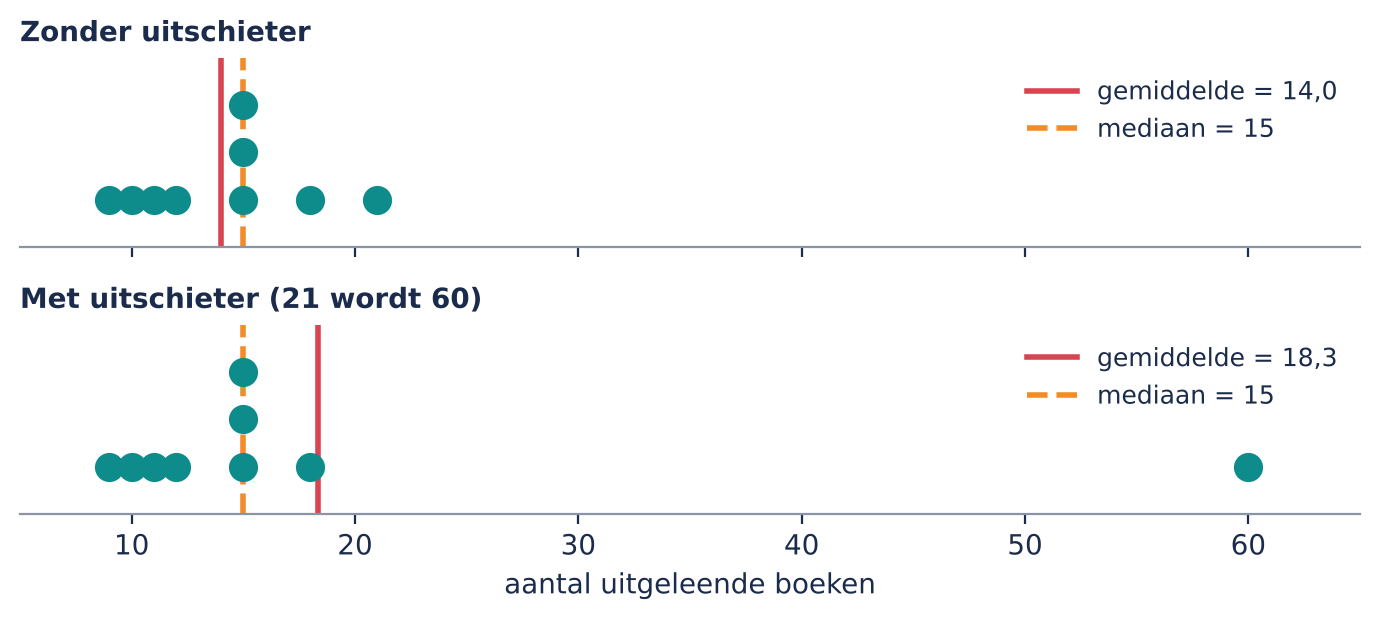
\includegraphics[width=0.75\textwidth]{figuren/l1_uitschieter.png}
\end{center}

\begin{letop}
\textbf{LET OP} \quad In het voorbeeld wordt 21 vervangen door 60. Het gemiddelde stijgt van 14,0 naar 18,3, terwijl de mediaan 15 blijft. Bij uitschieters (denk aan lonen of vermogens) geeft de mediaan vaak een eerlijker beeld van wat ‘typisch’ is.
\end{letop}

\subsection*{Theorie 1.3 · Gegroepeerde data}

\begin{theorie}
Bij een gegroepeerde frequentietabel ken je de exacte gegevens niet meer. Je werkt met het \textbf{klassenmidden}: $\dfrac{\text{ondergrens}+\text{bovengrens}}{2}$.

\begin{itemize}
\item Schatting van het gemiddelde: $\overline{x}\approx\dfrac{\sum(\text{klassenmidden}\cdot \text{AF})}{n}$.
\item De \textbf{modale klasse} is de klasse met de grootste AF. De \textbf{mediaanklasse} is de klasse waarin het middelste gegeven zit.
\end{itemize}

Notatie: de klasse [70, 75[ bevat alle waarden van 70 (inbegrepen) tot 75 (niet inbegrepen).
\end{theorie}

\subsection*{Aan de slag}

\subsubsection*{Oefening 1.1 \quad ★☆☆ \quad Stap voor stap}

Zeven tieners noteren hoeveel uur ze vorige week gamden: 12 – 5 – 8 – 20 – 8 – 15 – 8.

\textbf{a)} Rangschik de data van klein naar groot. \lijn

\textbf{b)} Bereken het gemiddelde. \lijn

\textbf{c)} Bepaal de mediaan. \lijn

\textbf{d)} Bepaal de modus. \lijn

\textbf{e)} Schrijf een zin die de mediaan interpreteert. \lijn

\begin{oplossing}
\textbf{Oplossing 1.1}

a) 5 – 8 – 8 – 8 – 12 – 15 – 20 \quad b) $\overline{x}=\dfrac{76}{7}\approx 10{,}9$ uur \quad c) Med = 8 uur (4de van 7 getallen) \quad d) Mod = 8 uur

e) De helft van de tieners gamede maximaal 8 uur, de andere helft minstens 8 uur.
\end{oplossing}

\subsubsection*{Oefening 1.2 \quad ★★☆ \quad Een even aantal gegevens}

De wachttijden (in minuten) van 8 patiënten bij de kinderarts: 17 – 9 – 22 – 6 – 13 – 18 – 11 – 16.

\textbf{a)} Bereken het gemiddelde en de mediaan. \lijn

\textbf{b)} Bepaal de modus. Wat valt je op? \lijn

\begin{oplossing}
\textbf{Oplossing 1.2}

Rangschikken: 6 – 9 – 11 – 13 – 16 – 17 – 18 – 22. a) $\overline{x}=\dfrac{112}{8}=14{,}0$ min; $\text{Med}=\dfrac{13+16}{2}=14{,}5$ min. b) Alle waarden komen even vaak voor (één keer), dus er is geen modus.
\end{oplossing}

\subsubsection*{Oefening 1.3 \quad ★★☆ \quad Context: zakgeld en een uitschieter}

Acht jongeren in een jeugdhuis noteren hun zakgeld per maand (in euro): 20 – 25 – 30 – 30 – 30 – 35 – 40 – 190.

\textbf{a)} Bereken het gemiddelde en de mediaan. \lijn

\textbf{b)} Welke centrummaat geeft het beste beeld van het ‘typische’ zakgeld? Waarom? \lijn

\textbf{c)} Bereken beide opnieuw zonder het bedrag van 190 euro. Welke centrummaat verandert nauwelijks? \lijn

\begin{oplossing}
\textbf{Oplossing 1.3}

a) $\overline{x}=\dfrac{400}{8}=50$ euro; Med = $\dfrac{30+30}{2}=30$ euro. b) De mediaan: ze ligt dicht bij bijna alle bedragen. Het gemiddelde (50 euro) wordt omhooggetrokken door de uitschieter 190 euro; geen enkele jongere heeft ongeveer 50 euro. c) Zonder 190: $\overline{x}=30$ euro en Med = 30 euro. Het gemiddelde daalt sterk (50 → 30), de mediaan verandert niet.
\end{oplossing}

\subsubsection*{Oefening 1.4 \quad ★★☆ \quad Categorische data}

Aan 40 ouders werd gevraagd hoe tevreden ze zijn over de buitenschoolse opvang.

\breedtes{50/25/25}
\begin{tabular}{lcc}
\hline
antwoord & AF & cumulatieve AF \\
\hline
zeer ontevreden & 1 & \\
ontevreden & 3 & \\
noch ontevreden, noch tevreden & 6 & \\
tevreden & 18 & \\
zeer tevreden & 12 & \\
\hline
\end{tabular}

\textbf{a)} Welk soort data is dit? \lijn

\textbf{b)} Vul de kolom cumulatieve AF aan (telkens optellen). Bepaal daarmee de mediaan. Tip: bij 40 gegevens zijn het 20ste en 21ste gegeven de middelste. \lijn

\textbf{c)} Bepaal de modus en schrijf een antwoordzin. \lijn

\textbf{d)} Waarom kan je hier geen gemiddelde berekenen? \lijn

\begin{oplossing}
\textbf{Oplossing 1.4}

a) Categorisch geordend. b) Cumulatief: 1 – 4 – 10 – 28 – 40. Het 20ste en 21ste gegeven zitten allebei in de groep ‘tevreden’: Med = tevreden. c) Mod = tevreden: de meeste ouders (18 van de 40) zijn tevreden over de opvang. d) Je kan niet optellen of delen met woorden; de afstand tussen ‘tevreden’ en ‘zeer tevreden’ is geen getal.
\end{oplossing}

\subsubsection*{Oefening 1.5 \quad ★★★ \quad Gegroepeerde data}

Bij een seniorennamiddag in een woonzorgcentrum noteert men de leeftijd van de 50 deelnemers.

\breedtes{30/30/20}
\begin{tabular}{lcc}
\hline
leeftijd (jaar) & klassenmidden & AF \\
\hline
[60, 65[ & & 4 \\
[65, 70[ & & 9 \\
[70, 75[ & & 15 \\
[75, 80[ & & 12 \\
[80, 85[ & & 7 \\
[85, 90[ & & 3 \\
\hline
\end{tabular}

\textbf{a)} Vul de kolom klassenmidden aan. \quad \textbf{b)} Schat het gemiddelde. \lijn

\textbf{c)} Geef de modale klasse en de mediaanklasse (het 25ste en 26ste gegeven zijn de middelste). \lijn

\textbf{d)} Is je antwoord bij b) exact? Verklaar. \lijn

\begin{oplossing}
\textbf{Oplossing 1.5}

a) 62,5 – 67,5 – 72,5 – 77,5 – 82,5 – 87,5. b) $\overline{x}\approx\dfrac{62{,}5\cdot 4+67{,}5\cdot 9+72{,}5\cdot 15+77{,}5\cdot 12+82{,}5\cdot 7+87{,}5\cdot 3}{50}=\dfrac{3715}{50}=74{,}3$ jaar. c) Modale klasse [70, 75[ (AF = 15). Cumulatief 4 – 13 – 28: het 25ste en 26ste gegeven zitten in [70, 75[, dat is ook de mediaanklasse. d) Nee, het is een schatting: we kennen de exacte leeftijden niet en gebruiken het klassenmidden.
\end{oplossing}

\subsubsection*{Oefening 1.6 \quad ★★★ \quad Context: terugrekenen met totalen}

Handig: \textbf{totaal = gemiddelde $\cdot$ aantal}.

\textbf{a)} Vijf begeleiders hebben een gemiddelde leeftijd van 30 jaar. Een nieuwe collega van 42 jaar komt erbij. Wat is nu de gemiddelde leeftijd? \lijn

\textbf{b)} Het gemiddelde op vier toetsen is 12 op 20. Hoeveel moet je op de vijfde toets halen om gemiddeld 13 te hebben? \lijn

\begin{oplossing}
\textbf{Oplossing 1.6}

a) Totaal vroeger: $5\cdot 30=150$. Nu: $\dfrac{150+42}{6}=32$ jaar. b) Gewenst totaal: $5\cdot 13=65$. Al behaald: $4\cdot 12=48$. Nodig: $65-48=17$ op 20.
\end{oplossing}

\subsection*{Invullen · de centrummaten}

\textbf{Woordenlijst:} gemiddelde – mediaan – modus – uitschieters – numerieke – centrummaat.

Een \gat{centrummaat} is een kengetal dat het centrum van de data weergeeft. Het \gat{gemiddelde} kan je enkel berekenen bij \gat{numerieke} data. De \gat{mediaan} is de middelste waarde van de gerangschikte gegevens. De \gat{modus} is de waarde die het vaakst voorkomt en is de enige centrummaat die je bij categorisch niet-geordende data kan gebruiken. Het gemiddelde is gevoelig voor \gat{uitschieters}.

\subsection*{Koppel · de beste centrummaat}

Welke centrummaat past het best bij de vraag? Kies \textbf{gemiddelde}, \textbf{mediaan} of \textbf{modus}.

\breedtes{75/25}
\begin{tabular}{ll}
\hline
Vraag & Centrummaat \\
\hline
a) Welke opvangvorm kiezen de meeste ouders (kinderdagverblijf, onthaalouder, grootouders)? & \\
b) Wat is het typische loon in een sector met enkele zeer hoge topsalarissen? & \\
c) Hoeveel uur verblijft een kind in de opvang als je de totale uren eerlijk over alle kinderen verdeelt? & \\
d) Wat is het ‘middelste’ antwoord op een tevredenheidsvraag van ‘zeer ontevreden’ tot ‘zeer tevreden’? & \\
\hline
\end{tabular}

\begin{oplossing}
\textbf{Oplossing Koppel}

a) modus \quad b) mediaan \quad c) gemiddelde \quad d) mediaan
\end{oplossing}

\subsection*{Foutjager}

Zoek de fout, leg uit waarom het fout is en verbeter.

\textbf{1.} Sara: ‘De mediaan van 3 – 9 – 1 – 7 – 5 is 1, want dat is het eerste getal.’ \lijn

\textbf{2.} Ahmed: ‘Bij 2 – 4 – 4 – 6 – 9 – 10 is de mediaan 4, want 4 komt het vaakst voor.’ \lijn

\textbf{3.} Lotte: ‘Het gemiddelde van de postcodes 9000 en 2000 is 5500, dus gemiddeld wonen onze leerlingen in 5500.’ \lijn

\begin{oplossing}
\textbf{Oplossing Foutjager}

1. Eerst rangschikken: 1 – 3 – 5 – 7 – 9, dus Med = 5. 2. Ahmed haalt mediaan en modus door elkaar. Mod = 4, maar $\text{Med}=\dfrac{4+6}{2}=5$. 3. Een postcode is een label (categorisch), geen hoeveelheid; een gemiddelde heeft hier geen betekenis.
\end{oplossing}

\subsection*{CHECK · Level 1}

De volgende getallen zijn het aantal vrijwilligersuren van zes jongeren: 4 – 7 – 7 – 9 – 10 – 13.

\textbf{1.} (3 p) Bereken het gemiddelde, de mediaan en de modus. \lijn

\textbf{2.} (2 p) Een zevende jongere doet 60 uur vrijwilligerswerk. Welke centrummaat verandert het meest? Verklaar. \lijn

\textbf{3.} (2 p) Bij welk soort data kan je de mediaan wel maar het gemiddelde niet berekenen? Geef een voorbeeld. \lijn

\begin{doel}
\textbf{Score:} \_\_\_ / 7 \quad ☐ behaald (vanaf 5 / 7) \quad ☐ nog even oefenen
\end{doel}

\begin{oplossing}
\textbf{Oplossing CHECK 1}

1. $\overline{x}=\dfrac{50}{6}\approx 8{,}3$ uur; $\text{Med}=\dfrac{7+9}{2}=8$ uur; Mod = 7 uur. 2. Het gemiddelde: het stijgt naar $\dfrac{110}{7}\approx 15{,}7$; de mediaan wordt 9 en de modus blijft 7. 3. Bij categorisch geordende data, bijvoorbeeld tevredenheid (zeer ontevreden … zeer tevreden).
\end{oplossing}
